%%%%%%%%%%%%%%%%%%%%%%%%%%%%%%%%%%%%%%%%%%%%%%%%%%%%%%%%%%%%%%%%%%%%%%%%%%%
% Chapter 6: Comparing more than two means
%%%%%%%%%%%%%%%%%%%%%%%%%%%%%%%%%%%%%%%%%%%%%%%%%%%%%%%%%%%%%%%%%%%%%%%%%%%

\Chapter{Chapter 6}{Comparing more than two means}{Chapter 6: Comparing more than two means}
{
Please read Chapter 14 and Chapter 16 from \textit{\href{https://learningstatisticswithr.com/}{{\color{black}Learning Statistics with R}}} before starting these assignments.
}

\fancyhead[R]{\fontsize{12}{14}\selectfont\textit{Chapter 6: Comparing more than two means}}

\chaptertitle{Chapter 6: Comparing more than two means}

\learningobjectives{
    \item Implementing a t-test as a regression in R
    \item Performing an ANOVA in R
    \item Implementing an ANOVA as a regression in R
    \item Introducing a covariate in ANCOVA in R
}

% To add an assignment to the chapter, create a file in the folder "Assignments" and insert the link below

%%%%%%%%%%%%%%%%%%%%%%%%%%%%%%%%%%%%%%%%%%%%%%%%%%%%%%%%%%%%%%%%%%%%%%%%%%%
% Assignment 6.1: Implementing a t-test as a regression in R
%%%%%%%%%%%%%%%%%%%%%%%%%%%%%%%%%%%%%%%%%%%%%%%%%%%%%%%%%%%%%%%%%%%%%%%%%%%

\rassignment{Assignment 6.1: Implementing a t-test as a regression in R}

Many of the statistical tests that we have seen are actually equivalent to a specific form of \concept{linear regression}. To understand how a \concept{t-test} can be implemented as a \concept{linear regression}, let’s look at an example. Suppose you work in advertising and show four groups of people an advertisement, where the only difference is in the color/position of the eyes of the model (blue eyes, brown eyes, green eyes, or downward-looking eyes), and you ask them how they rate your brand after seeing this advertisement. For this assignment, we will use the \dataset{eyeColor.csv} data file that contains 222 participants’ ratings for one of the four groups. As a first question, you want to assess whether there is a difference in the ratings if the model shown in the advertisement has blue eyes rather than brown eyes. \\

\question{
    6.1 a
}{
    Read in the file \dataset{eyeColor.csv} and store the data in an object called \rcode{dataset8}.
}

\rcodeanswertiny{6.1a}

Note that this data set contains all four groups (\rcode{Blue}, \rcode{Brown}, \rcode{Green}, \rcode{Down}). Run the following \texttt{R} code to isolate the scores of the groups that were shown advertisements with \rcode{Blue} and \rcode{Brown} eyes and store them in the new \rcode{ttestData} object. \\

\codeblock{ttestData  <- subset(dataset8,\\ 
                     \hspace*{110pt}dataset8\$Group == \textquotesingle Blue\textquotesingle | \\
                     \hspace*{110pt}dataset8\$Group == \textquotesingle Brown\textquotesingle)}

\question{
    6.1 b
}{
    Write down the \concept{null hypothesis} $H_0$ and \concept{alternative hypothesis} $H_1$ for testing whether the \concept{mean} score of the group that was shown \rcode{Blue} eyes is equal to the \concept{mean} score of the group that was shown \rcode{Brown} eyes. Remember that these are independent \concept{samples}.
}

\hypothesesbox{6.1b}

\question{
    6.1 c
}{
    Use the \rcode{t.test()} function to test the equality of the two means.
}

\hint{Hint 6.1: Make sure to specify \rcode{var.equal = TRUE} to perform a \concept{two-sample t-test} instead of the non-parametric \concept{Welch’s t-test}.}

\rcodeanswertiny{6.1c}

\question{
    6.1 d
}{
    What is your conclusion on the basis of these results? Include the following elements:
        \begin{itemize}
        \item[$\square$] Discuss what the \concept{p-value} is for this test.
    \item[$\square$] Discuss whether $H_0$ is rejected or not.
    \item[$\square$] Describe what this tells us about $\mu_{Blue}$ and $\mu_{Brown}$.  
    \item[$\square$] Describe what type of error is relevant \textit{(type-I or type-II)}.
\end{itemize}
}

\sixlineanswerbox{6.1d}

Now, instead of using the \rcode{t.test()} function to test the equality of the two \concept{means}, you can test the equality of the two \concept{means} using a \concept{regression model}. Therefore, you need to add a variable to our data that says whether a participant saw one of the two groups (e.g., only the people that were shown \rcode{Brown} eyed models). \\

Run the following code in R: \\

\codeblock{dummyBrown <- as.numeric(ttestData\$Group == \textquotesingle Brown\textquotesingle)\\
ttestData <- cbind(ttestData, dummyBrown)}

\clearpage % Page break

\question{
    6.1 e
}{
    What are the contents of \rcode{dummyBrown}? What do we call this kind of variable?
}

\twolineanswerbox{6.1e}

\question{
    6.1 f
}{
    Create a \concept{linear model} in \texttt{R} where you predict the (outcome) variable \rcode{Score} using only the (predictor) variable \rcode{dummyBrown}. Store the fitted model in an object called \rcode{ttestreg}.
}

\rcodeanswersmall{6.1f}

\question{
    6.1 g
}{
    Use the \rcode{summary()} function to inspect the results of the \rcode{ttestreg} model. How does this output correspond to the \concept{t-test} that you performed in assignment 6.1c? Where do you find the \concept{p-value} that you calculated using the \rcode{t.test()} function?
}

\rcodeanswersmall{6.1g}

\twolineanswerbox{6.1g}

\clearpage % Page break
%%%%%%%%%%%%%%%%%%%%%%%%%%%%%%%%%%%%%%%%%%%%%%%%%%%%%%%%%%%%%%%%%%%%%%%%%%%
% Assignment 6.2: Performing an ANOVA in R
%%%%%%%%%%%%%%%%%%%%%%%%%%%%%%%%%%%%%%%%%%%%%%%%%%%%%%%%%%%%%%%%%%%%%%%%%%%

\rassignment{Assignment 6.2: Performing an ANOVA in R}

Now let’s extend the analysis from assignment 6.1 by comparing all four groups (\rcode{Blue}, \rcode{Brown}, \rcode{Green}, \rcode{Down}) instead of only the \rcode{Blue} and \rcode{Brown} groups. When you are testing more than two \concept{means}, you can use an \concept{ANOVA} test (a specific form of regression). Since you want to compare all four groups, you can leave the \rcode{ttestData} from the previous assignment and focus on the data in \rcode{dataset8}. Remember that you are interested in testing the effect of the model’s eye color on the rating of your brand. \\

\question{
    6.2 a
}{
    Write down the \concept{null hypothesis} $H_0$ and the \concept{alternative hypothesis} $H_1$ for testing whether the \concept{mea}n score of the four groups (\rcode{Blue}, \rcode{Brown}, \rcode{Green}, \rcode{Down}) are equal.
}

\hypothesesbox{6.2a}

The \concept{ANOVA} uses the \concept{F-distribution} to test for a significant difference between all four \concept{means}. Using the (two types of) \concept{degrees of freedom} of this \concept{F-distribution}, you can calculate the \concept{critical F-value} that is required to reject the \concept{null hypothesis} that the \concept{means} of the four groups are equal. Table 5 on page~\pageref{table5} contains the \concept{critical F-values} for a confidence of 95\%.
\vspace*{.5cm}
\begin{center}
    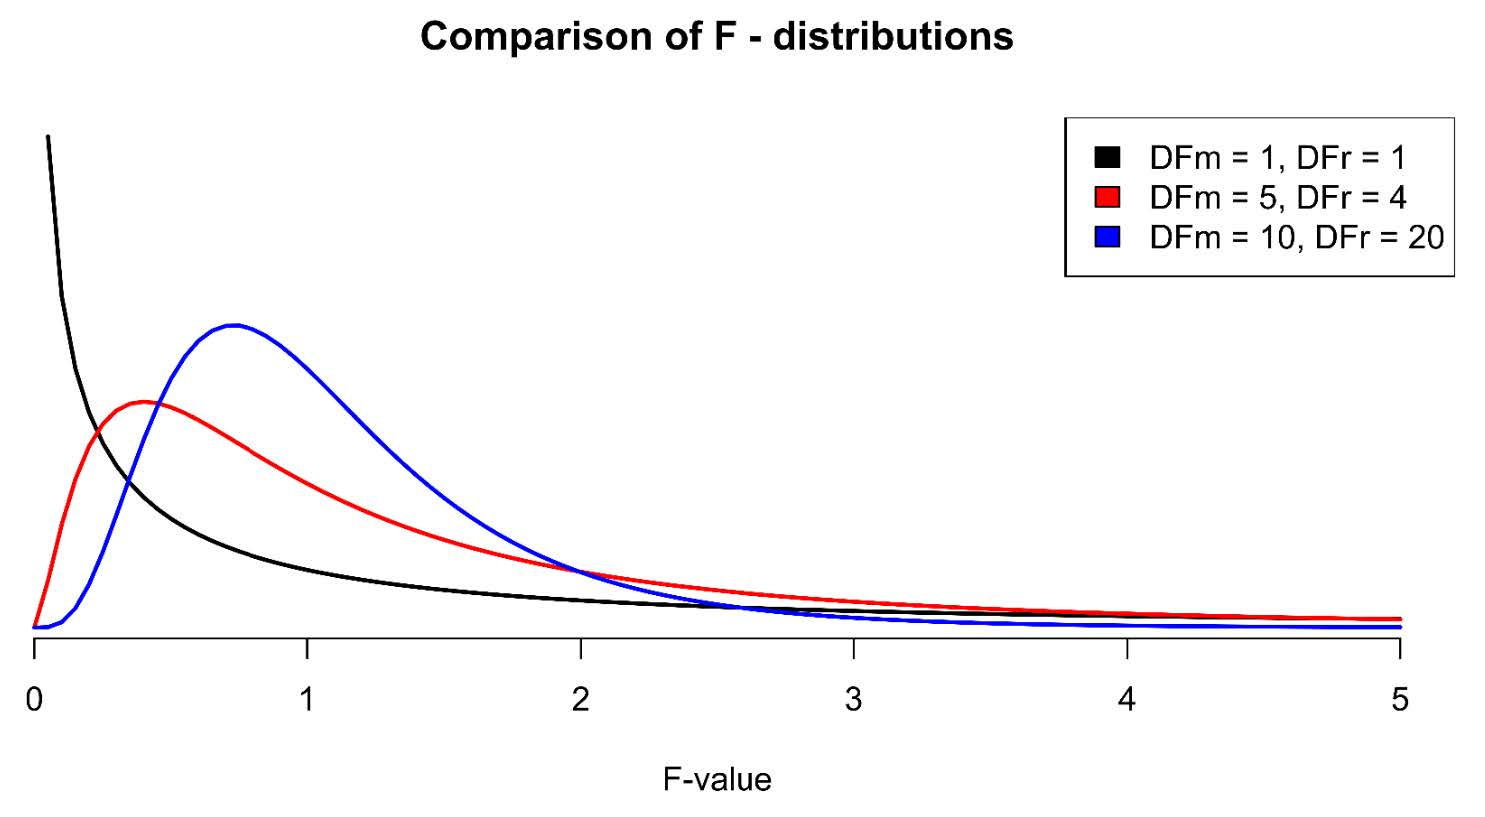
\includegraphics[width=.9\textwidth]{Files/Images/fdistributions.jpg}
\end{center}

\clearpage % Page break

\question{
    6.2 b
}{
    Calculate the \concept{degrees of freedom} $df_M$ and $df_R$ of the \concept{F-distribution} for the data in \rcode{dataset8}.
}

\hint{Hint 6.2: You can find the formulas for $df_M$ and $df_R$ in the formula sheet.}

\emptyanswerbox{
    6.2b
}{
    $df_M$: \shortanswerline \hspace*{3cm} $df_R$: \shortanswerline
}

\question{
    6.2 c
}{
    Using the \rcode{qf()} function, calculate the \concept{critical F-value} that is required to reject the \concept{null hypothesis} $H_0$ for these data with 95\% confidence.
}

\rcodeanswertiny{6.2c}

\emptyanswerbox{
    6.2c
}{
    Critical F-value: \shortanswerline
}

The \rcode{aov()} function in \texttt{R} is a wrapper for the \rcode{lm()} function. The difference between these two functions is that the \rcode{lm()} function can only handle \concept{categorical} predictors with two levels (e.g., a \concept{dummy variable}). The \rcode{aov()} function can handle \concept{categorical} predictor variables with more than two levels, since it automatically rewrites the \rcode{formula} to include the \concept{dummy variables}. \\ 

\question{
    6.2 d
}{
    Use the \rcode{aov()} function to perform an \concept{ANOVA} with the dependent (outcome) variable \rcode{Score} and the independent (predictor) variable \rcode{Group} and store the result in an object named \rcode{anovaResult}.
}

\hint{Hint 6.3: You can check more information on the \rcode{aov()} function with \rcode{?aov}.}

\rcodeanswersmall{6.2d}

\clearpage % Page break

\question{
    6.2 e
}{
    Use the \rcode{summary()} function to inspect the results of the \concept{ANOVA} in \rcode{anovaResult}. What is the \concept{F-value} that is calculated from the \concept{sample}? What is the \concept{p-value} calculated from the \concept{sample}?
}

\rcodeanswertiny{6.2e}

\emptyanswerbox{
    6.2e
}{
    F-value: \shortanswerline \hspace*{3cm} p-value: \shortanswerline
}

\question{
    6.2 f
}{
    What is your conclusion on the basis of these results? Include the following elements:
        \begin{itemize}
        \item[$\square$] Discuss what the \concept{p-value} is for this test.
    \item[$\square$] Discuss whether $H_0$ is rejected or not.
    \item[$\square$] Describe what this tells us about $\mu_{Blue}$, $\mu_{Brown}$, $\mu_{Green}$, and $\mu_{Down}$.  
    \item[$\square$] Describe what type of error is relevant \textit{(type-I or type-II)}.
\end{itemize}
}

\sixlineanswerbox{6.2f}

\clearpage % Page break
%%%%%%%%%%%%%%%%%%%%%%%%%%%%%%%%%%%%%%%%%%%%%%%%%%%%%%%%%%%%%%%%%%%%%%%%%%%
% Assignment 6.3: Implementing an ANOVA as a regression in R
%%%%%%%%%%%%%%%%%%%%%%%%%%%%%%%%%%%%%%%%%%%%%%%%%%%%%%%%%%%%%%%%%%%%%%%%%%%

\rassignment{Assignment 6.3: Implementing an ANOVA as a regression in R}

Now that you have seen the results of the \concept{ANOVA}, let’s try to replicate these by implementing the same \concept{ANOVA} as a \concept{linear regression}. Remember that this is exactly what you did for the \concept{t-test} in assignment 6.1 by adding one \concept{dummy variable} to your model that isolated the \rcode{Brown} group. For the \concept{ANOVA}, you are going to have three \concept{dummy variables} in your model, one that represents  \rcode{Brown} eyes, one that represents \rcode{Blue} eyes, and one that represents \rcode{Green} eyes. You first have to add these dummy variables to your data set. \\

Run the following code in \texttt{R} that adds a \concept{dummy variable} for \rcode{Brown} eyes to the data set: \\

\codeblock{dummyBrown <- as.numeric(dataset8\$Group == \textquotesingle Brown\textquotesingle) \\
dataset8   <- cbind(dataset8, dummyBrown)}

\question{
    6.3 a
}{
    Add two more \concept{dummy variables} to the data in \rcode{dataset8}, one for \rcode{Blue} eyes and one for \rcode{Green} eyes. Name these variables \rcode{dummyBlue} and \rcode{dummyGreen}.
}

\rcodeanswermedium{6.3a}

\question{
    6.3 b
}{
    Create a \concept{linear model} in \texttt{R} where you predict the (outcome) variable \rcode{Score} using the (predictor) variables \rcode{dummyBrown}, \rcode{dummyGreen}, and \rcode{dummyBlue}. Store the fitted \concept{linear model} in an object called \rcode{anovaReg}.
}

\rcodeanswersmall{6.3b}

\question{
    6.3 c
}{
    Use the \rcode{summary()} function to inspect the results of the \concept{linear model} stored in \rcode{anovaReg}. What is the \concept{F-value} of the model? What is the \concept{p-value} of this model?
}

\rcodeanswertiny{6.3c}

\emptyanswerbox{
    6.3c
}{
    F-value: \shortanswerline \hspace*{3cm} p-value: \shortanswerline
}

\clearpage % Page break

\question{
    6.3 d
}{
    Do the \concept{F-value} and \concept{p-value} of this \concept{linear model} match those of the \concept{ANOVA} in assignment 6.2?
}

\emptyanswerbox{
    6.3d
}{
    \vspace*{-15pt}
    \begin{center}
        YES / NO
    \end{center}
}

\clearpage % Page break
%%%%%%%%%%%%%%%%%%%%%%%%%%%%%%%%%%%%%%%%%%%%%%%%%%%%%%%%%%%%%%%%%%%%%%%%%%%
% Assignment 6.4: Introducing a covariate in ANCOVA in R
%%%%%%%%%%%%%%%%%%%%%%%%%%%%%%%%%%%%%%%%%%%%%%%%%%%%%%%%%%%%%%%%%%%%%%%%%%%

\rassignment{Assignment 6.4: Introducing a covariate in ANCOVA in R}

There might be other determinants that influence people’s ratings of your brand that you have not captured by varying the eye color in the advertisements. An example of this might be people’s initial rating of your brand. These kinds of variables are called \concept{covariates} and you can incorporate them in our \concept{ANOVA}, very smoothly resulting in an \concept{ANCOVA}. In our scenario, we want to incorporate the \concept{covariate} for the initial score that our raters gave by adding the \rcode{initialScore} variable to our \concept{linear model}. \\

\question{
    6.4 a
}{
    Create a \concept{linear model} in \texttt{R} where you predict the (outcome) variable \rcode{Score} using the (predictor) variables \rcode{dummyBrown}, \rcode{dummyGreen}, \rcode{dummyBlue}, and the variable \rcode{initialScore}. Store the fitted model in an object called \rcode{ancovaReg}.
}

\rcodeanswersmall{6.4a}

\question{
    6.4 b
}{
    Use the \rcode{summary()} function to inspect the results of the \concept{linear model} stored in \rcode{ancovaReg}. What is the \concept{F-value} of the model? What is the \concept{p-value} of this model?
}

\rcodeanswertiny{6.4b}

\emptyanswerbox{
    6.4b
}{
    F-value: \shortanswerline \hspace*{3cm} p-value: \shortanswerline
}

\question{
    6.4 c
}{
    What is your conclusion on the basis of these results? Include the following elements:
        \begin{itemize}
        \item[$\square$] Discuss what the \concept{p-value} is for this test.
    \item[$\square$] Discuss whether $H_0$ is rejected or not.
    \item[$\square$] Describe what this tells us about $\mu_{Blue}$, $\mu_{Brown}$, $\mu_{Green}$, and $\mu_{Down}$, given the covariate.  
    \item[$\square$] Describe what type of error is relevant \textit{(type-I or type-II)}.
\end{itemize}
}

\threelineanswerbox{6.4c}

\clearpage % Page break

\question{
    6.4 d
}{
    Can you tell whether \rcode{initialScore} is a good predictor of the \rcode{Score}? On what value can you base your conclusion?
}

\hint{Hint 6.4: First consider which results you would expect if $\beta_3 \neq 0$.}

\twolineanswerbox{6.4d}

To find out whether adding this \concept{covariate} is an improvement over the \concept{linear model} in assignment 6.3, we can compare the two \concept{linear models} \rcode{anovaReg} (without \rcode{initialScore}) and \rcode{ancovaReg} (with \rcode{initialScore}) with respect to their proportion of \concept{explained variance} (their $R^2$).  \\

\question{
    6.4 e
}{
    What is the (multiple) $R^2$ of the \rcode{anovaReg} \concept{model}? What is the (multiple) $R^2$ of the \rcode{ancovaReg} \concept{model}? Which \concept{model} explains more variation in the outcome variable \rcode{Score}?
}
    
\emptyanswerbox{
    6.4e
}{
    $R^2$ \rcode{anovaReg}: \shortanswerline \hspace*{1cm} $R^2$ \rcode{ancovaReg}: \shortanswerline
    \answerskip
    The \rcode{anovaReg} / \rcode{ancovaReg} regression model explains more variation in the outcome variable score.
}

\question{
    6.4 f
}{
    Interpret the $R^2$ for the best model.
}

\twolineanswerbox{6.4f}

The $R^2$ statistic will always increase when you add more (predictor) variables to our \concept{model}, since you are adding more information. To reliably compare our two \concept{models}, you have to look at a measure that penalizes a \concept{model} for including more (predictor) variables. You can use the \concept{AIC} value for that. The rule of thumb for the \concept{AIC} value is that the \concept{model} with the lower \concept{AIC} value is the preferred model. \\

\clearpage % Page break

\question{
    6.4 g
}{
    Use the \rcode{AIC()} function to calculate the \concept{AIC} value of the \rcode{anovaReg} and the \rcode{ancovaReg} models.
}

\rcodeanswersmall{6.4g}

    
\emptyanswerbox{
    6.4g
}{
    AIC \rcode{anovaReg}: \shortanswerline \hspace*{.5cm} AIC \rcode{ancovaReg}: \shortanswerline
}

\question{
    6.4 h
}{
    What is the preferred model? How can you use the \concept{AIC} statistic to validate you answer in assignment 6.4d?
}

\twolineanswerbox{6.4h}

\clearpage % Page break
%%%%%%%%%%%%%%%%%%%%%%%%%%%%%%%%%%%%%%%%%%%%%%%%%%%%%%%%%%%%%%%%%%%%%%%%%%%
% Assignment 6.5: Using post-hoc tests to find differences in means
%%%%%%%%%%%%%%%%%%%%%%%%%%%%%%%%%%%%%%%%%%%%%%%%%%%%%%%%%%%%%%%%%%%%%%%%%%%

\rassignment{Assignment 6.5: Using post-hoc tests in R to find differences in means}

For this assignment you will have to download the data file \dataset{iowa.RData} from the online resources\footnote{These data are taken from \url{https://data.iowa.gov/State-Government-Finance/State-of-Iowa-Checkbook/cyqb-8ina}.}. \dataset{.RData} files are compressed \texttt{R} objects, and are useful when dealing with very large data sets such as this one. \\

The \dataset{iowa.RData} file contains payment transactions recorded in the State of Iowa’s central accounting system for the Executive Branch and is real data. \\

\question{
    6.5 a
}{
    Load the \dataset{iowa.RData} data file into the environment using the \rcode{load()} function. 
}

\rcodeanswertiny{6.5a}

The data set is now stored in object called \rcode{iowa}. \\

\question{
    6.5 b
}{
    Give a short description of the data in \rcode{iowa}.
}

\hint{Hint 6.5: Search the internet for the source of these data to find out what the columns represent.}

\threelineanswerbox{6.5b}

\question{
    6.5 c
}{
    How many rows and columns does the \rcode{iowa} data set have?
}

\emptyanswerbox{
    6.5c
}{
    Rows: \shortanswerline \hspace*{3cm} Columns: \shortanswerline
}

\clearpage % Page break

\question{
    6.5 d
}{
    How many unique services are there? Make a \concept{frequency table} of these services.
}

\rcodeanswertiny{6.5d}

\emptyanswerbox{
    6.5d
}{
    Unique services: \shortanswerline 
}

\question{
    6.5 e
}{
    Which service has the most rows? How many rows does this service have?
}

\emptyanswerbox{
    6.5e
}{
    Service: \shortanswerline \hspace{3cm} Rows: \shortanswerline
}

\question{
    6.5 f
}{
    How many rows show a difference in invoice date and payment date?
}

\rcodeanswertiny{6.5f}

\emptyanswerbox{
    6.5f
}{
    Number of rows that show a difference: \shortanswerline 
}

\question{
    6.5 g
}{
    Create a new data set that consists of these differences, and name the new data set \rcode{dataDif}.
}

\rcodeanswermedium{6.5g}

\clearpage % Page break

\question{
    6.5 h
}{
    Create an extra column named \rcode{dif.days} in \rcode{dataDif} that contains the number of days between invoice and payment.
}

\hint{Hint 6.6: Make sure that the column \rcode{dif.days} is numeric.}

\rcodeanswertiny{6.5h}

\question{
    6.5 i
}{
    Calculate the \concept{minimum}, \concept{maximum}, \concept{mean}, \concept{quartiles}, and \concept{standard deviation} of the column \rcode{dif.days}.
}

\rcodeanswermedium{6.5i}

\emptyanswerbox{
    6.5i
}{  
    Minimum: \quad \shortanswerline \quad Upper quartile: \quad \quad \shortanswerline
            \answerskip
            Mean: \quad\hspace*{9pt} \shortanswerline \quad \quad Lower quartile: \quad \quad \shortanswerline
            \answerskip
            Maximum: \quad \shortanswerline \quad Standard deviation: \shortanswerline
}

\question{
    6.5 j
}{
    Create a histogram of the column \rcode{dif.days}. Describe what you see in the histogram.
}

\rcodeanswertiny{6.5j}
\onelineanswerbox{6.5j}

\clearpage % Page break

\question{
    6.5 k
}{
    Again, create a histogram, but now only use the subset of \rcode{dif.days} that is in the 5-95\% quantile range (so you cut off the bottom and top 5\%).
}

\hint{Hint 6.7: Hint: use the \rcode{quantile} function.}

\rcodeanswersmall{6.5k}

You don't trust the negative values in \rcode{dif.days} as you cannot interpret them, and therefore you will not include them in your investigation. Moreover, you also don't want to include value in \rcode{dif.days} that are higher than 365 days. \\

\question{
    6.5 l
}{
    Create a new data set in which these values are removed and name this data set \rcode{dataDif2}.
}

\rcodeanswertiny{6.5l}

\question{
    6.5 m
}{
    Create a scatter plot with \rcode{dif.days} on the \textit{y-axis} and \rcode{Amount} on the \textit{x-axis}.
}

\rcodeanswertiny{6.5m}

\question{
    6.5 n
}{
    Compute the \concept{correlation} between the time between invoice and payment, and the amount that is paid.
}

\rcodeanswertiny{6.5n}
\emptyanswerbox{
    6.5n
}{
    Correlation: \shortanswerline 
}

\clearpage % Page break

\question{
    6.5 o
}{
    Elaborate on the \concept{correlation coefficient} and it's significance. What does this imply?
}

\threelineanswerbox{6.5o}

\question{
    6.5 p
}{
    Compute the \concept{mean} \rcode{dif.days} per expense category.
}

\hint{Hint 6.8: Use the \rcode{aggregate()} function (for more help on this function see \rcode{?aggregate}).}

\rcodeanswertiny{6.5p}
\twolineanswerbox{6.5p}

\question{
    6.5 q
}{
    Use the \rcode{aov()} function to test whether the \concept{means} that you computed in assignment 6.5p are statistically different.
}

\emptyanswerbox{
    6.5 q
}{
p-value: \shortanswerline
\answerskip
Conclusion:
\answerskip
\rule{\textwidth}{0.4pt}
}

\rcodeanswertiny{6.5q}

\clearpage % Page break

\question{
    6.5 r
}{
    Use \concept{Tukey's Honest Significant Differences} to find out which group \concept{means} are truly different.
}

\hint{Hint 6.9: Use the \rcode{TukeyHSD()} function to find \concept{Tukey's Honest Significant Differences}.} 

\rcodeanswertiny{6.5r}

\twolineanswerbox{6.5r}

In assignment 6.5q you have computed an \concept{ANOVA}, but this is statistically not completely sound. \\

\question{
    6.5 s
}{
    Can you formulate why the \concept{ANOVA} in assignment 6.5q was not statistically sound? What would be an appropriate analysis?
}

\twolineanswerbox{6.5s}

\question{
    6.5 t
}{
    Why do you think it is a good or bad idea to calculate \concept{p-values} if the number of rows in the data is large?
}

\threelineanswerbox{6.5t}

\clearpage % Page break